% vim: nospell
\input set/preamble.tex
\input set/macros.tex
\input set/listings.tex

\begin{document}

% Front matter %%%%%%%%%%%%%%%%%%%%%%%%%%%%%%%%%%%%%%%%%%%%%%%%%%%%%%%%%%%%%%%%%
\pagenumbering{roman}
\pagestyle{empty}
\input set/frontpage
\input set/titlepage
\pagestyle{fancy}
\setcounter{page}{1}
\tableofcontents
\cleardoublepage

% Main matter %%%%%%%%%%%%%%%%%%%%%%%%%%%%%%%%%%%%%%%%%%%%%%%%%%%%%%%%%%%%%%%%%%
\setcounter{page}{1}
\pagenumbering{arabic}

% Intro
\chapter{Introduction}
\label{cha:intro}
Smartphones and the need for high data rates have become an integrated part of the our everyday lives. The focus on data rates have become apparent with the standardization fo the 4th Generation (4G) of mobile communications, featuring Long Term Evolution (LTE) and LTE-Advanced (LTE-A) which both are to increase the data throughput. 

The specifications of 4G increase the number of antennas (MIMO), extend the bandwidth and define Carrier Aggregation (CA) combinations, among others. The operating frequencies for 4G are scattered around, ranging from \SIrange{698}{2690}{MHz}. Developing small handset antennas that can cover all these bands is a challenge for the antenna engineers, particularly for the lower bands, due to the fundamental limits and trade-offs between size, bandwidth and efficiency\cite{}. However the lower bands offer attractive features such as high building penetration and wide range cell-coverage. 

One way to overcome this problem is by using frequency-reconfigurability, to achieve good efficiency in the low bands and increase the number of bands that can be covered. Tuning can be performed on the antenna feeding line \cite{} \cite{} or on the antenna element \cite{} \cite{}. In this project MEMS tunable capacitors are used, since they offer low insertion loss, high voltage handling, and low power consumption\cite{}. Furthermore, the project aims to develop tunable antennas supporting MIMO operation on LTE bands for a handset. 
\fixme{Update cites}

\section{Reading Guidelines}
Throughout the report, a lot of sweep-plots will be presented with many plots per figure. The color order presented in Figure~\ref{fig:colororder} is used for all sweeps so the first plot is always blue, the next is green, and so forth.

\definecolor{bb}{rgb}{0.0, 0.0, 1.0}
\definecolor{gg}{rgb}{0.0, 0.5, 0.0}
\definecolor{rr}{rgb}{1.0, 0.0, 0.0}
\definecolor{cc}{rgb}{0.0, 0.75, 0.75}
\definecolor{mm}{rgb}{0.75, 0.0, 0.75}
\definecolor{yy}{rgb}{0.75, 0.75, 0.0}
\definecolor{kk}{rgb}{0.0, 0.0, 0.0}
\begin{figure}[htbp]
    \centering
    \begin{tikzpicture}[scale=0.5]
        \foreach \x/\c in {1/bb, 2/gg, 3/rr, 4/cc, 5/mm, 6/yy, 7/kk} {
            \fill[\c] (\x, 0) rectangle ++(1,1);
            \path (\x,1) ++ (right:0.5) node[above] {\x};
        };
    \end{tikzpicture}
    \caption{Color order for sweep plots in the report.}
    \label{fig:colororder}
\end{figure}

When two-port S-parameter measurements are mentioned in the report, port 1 is always the top-antenna and port 2 is the side-antenna unless otherwise noted.


\section{Initiating Problem}
\label{sec:init_problem}


% Analysis
\chapter{Post Processing}
\label{cha:postproc}

In this chapter, the libraries for post processing data from CST and Satimo will be described. The libraries are written in Python. By the end of the chapter, usage examples will be given.

\section{Data Format}
The trx files, from Satimo Passive Measurement, contain data formatted in four columns:
\begin{enumerate}
    \item Horizontal polarization, real part.
    \item Horizontal polarization, imaginary part.
    \item Vertical polarization, real part.
    \item Vertical polarization, imaginary part.
\end{enumerate}
Each column contains 
\begin{equation}
    n_r =  n_f \times n_a \times n_e
\end{equation}
where
\begin{where}
\item[$n_r$] Total number of rows per column.
\item[$n_f$] Number of different frequencies in the measurement.
\item[$n_a$] Number of azimuth coordinates (usually 8).
\item[$n_e$] Number of elevation coordinates (usually 15).
\end{where}
The first $n_a \times n_e$ rows are for the first frequency and the next $n_a \times n_e$ rows are for the second frequency. Within this, the first $n_e$ rows are for the first azimuth angle and so on.

To get a better overview, the basic format for the following libraries is a $\theta \times \phi$-matrix like the following:
\begin{equation}
    M = \begin{bmatrix}
        m_{1,1} & m_{1,2} & \dots & m_{1,n} \\
        m_{2,1} & m_{2,2} & \dots & m_{2,n} \\
        \vdots & \vdots & & \vdots \\
        m_{m,1} & m_{m,2} & \dots & m_{m,n}
    \end{bmatrix}
\end{equation}
The data is rearranged to have $\phi$ go from \ang{0} to \ang{360} and $\theta$ from \ang{0} to \ang{180} as shown in Table~\ref{tab:matrixformat}.

\begin{table}[htbp]
    \centering
    \begin{tabular}{|l|c|c|}
        \hline
        Elements & $\theta$ & $\phi$ \\
        \hline
        $m_{1,1}$ & \ang{0} & \ang{0} \\
        $m_{1,n}$ & \ang{0} & $\ang{360}$ \\
        $m_{m,1}$ & \ang{180}$^{\dagger}$ & \ang{0} \\
        \hline
    \end{tabular}
    \caption{Format of $\theta\times\phi$-matrix. $^{\dagger}$For Satimo measurements, this is $180-22.5=\ang{157.5}$ because of the blind spot in the bottom.}
    \label{tab:matrixformat}
\end{table}

\section{Basic Antenna Parameters}
This section will give a summery of the fundamental theories and parameters that are used to describe antennas. This should give a basic understanding of antennas and the parameters described in this section are used throughout the report. 

\subsection{Antenna Definition}
\label{subsec:antenna-def}
The IEEE defines an antenna as: ``a means for radiating or receiving radio waves''. In other words, the purpose of an antenna is to make the transistion from a signal in a transmission line to electromagnetic fields in the air. An antenna will radiates an electric field (E-field) in a given direction, which then induces a magnetic field (H-field) orthogonal to the E-field, this relation is described by Maxwell's Equations which is covered in Section~\ref{sec:fdtd}. \cite{}

\subsection{Isotropic Radiator}
\label{subsec:isotropic-ant}
An isotropic antenna, can be represented as a point source. The isotropic antenna radiates its power uniformly in a sphere. The power density $S_{iso}$ can be expressed as the source power $P_s$ over the surface area of a sphere which is given by $4\pi r^2$. \cite{} 

\begin{align}
  S_{iso} = \frac{P_s}{4\pi r^2}
\end{align}

Clearly it is not possible to construct such an antenna, however it is used as a reference for quantifying other properties of the antenna. These properties could be the gain or directivity (See Section\ref{subsec:dir_gain}), and the unit would then be in \si{dBi} rather than \si{dB}.

\subsection{Radiation Pattern}
\label{subsec:radiation-p}
The radiation pattern describes how the antenna emits or receives radiated power. This is commonly visualized by a 3D plot or 2D cuts of the 3D plot in specific coordinates. The unit of power used is often gain or directivity (See Section~\ref{subsec:dir_gain}) and this is often compared to the isotropic antenna. \cite{}

\subsection{Field Regions}
The waves transmitted from the antenna are usually grouped into three regions of radiation, based on how the waves propagate and the field structure\cite{balanis2012antenna}. Obviously there is no abrupt change, but rather a continuous change.

\begin{itemize}
\item The Reactive near-field 
\item The Radiating near-field (Fresnel)
\item The Far-field
\end{itemize}

The reactive near-field is defined as the portion of the near-field region immediately surrounding the antenna wherein the reactive field predominates\cite{balanis2012antenna}. The outer boundary for this region is given by $R < 0.62 \sqrt{\frac{D^3}{\lambda}}$\cite{balanis2012antenna}.

The radiating near-field is defined as the region between the reactive near-field and the far-field, this field might not exist in the case that the overall antenna dimension is very small compared to the wavelength. The outer boundary for this is defined as $R \geq \frac{2D^2}{\lambda}$\cite{balanis2012antenna}.

The far-field region is defined as the region of the field where the angular field distribution is independent of the distance, that is the radiation pattern does not change shape with distance. The far-field is also dominated by fields where the E- and H-fields are orthogonal and propagates as plane waves. The inner boundary is given as $R = \frac{2D^2}{\lambda}$\cite{balanis2012antenna}.

These different regions are illustrated on Figure~\ref{fig:field-regions}. 

\begin{figure}[htbp]
  \centering
  \includegraphics[scale=1]{img/analysis/radiationfields}
  \caption{Visualization of different fields \cite{balanis2012antenna}.}
  \label{fig:field-regions}
\end{figure}

\subsection{Directivity and Gain}
\label{subsec:dir_gain}
Directivity is defined as the ratio of the power radiated at a  point with a certain angle and distance from the antenna compared to what would be radiated from a reference isotropic antenna. Mathematically it can be written as \cite{}: 
\begin{align}
  D = \frac{U}{U_0} = \frac{4 \pi U}{P_{rad}} 
\end{align}
where
\begin{where}
  \item[$D$] is the directivity
  \item[$U$] is the radiation intensity
  \item[$U_0$] is the radiation intensity of an isotropic source
  \item[$P_{rad}$] is the total radiated power 
\end{where}
It should be noted, that for this equation to be valid, the waves must propagate as plane waves, thus being in the far-field region.


Gain is a measure closely related to directivity, it takes the antenna efficiency of the antenna into account as well as the direction. The gain is defined as the ratio of the intensity in a given direction to the radiant intensity that would be obtained if it was radiated isotropically. In mathematical form it can be expressed as \cite{}:

\begin{align}
  G = 4 \pi \frac{\text{radiation intensity}}{\text{total accepted input power}} = 4 \pi \frac{U(\theta,\phi)}{P_{in}}
\end{align}

In many cases the relative gain is used, which is defined as the ratio of the power gain in a given direction to the power gain of a reference antenna in its referenced direction. The reference antenna could be a dipole, horn etc. 

The gain can also be calculated using the directivity, since they are only related by the efficiency. This is given as: \cite{}

\begin{align}
  G(\theta,\phi) = e_{cd}D(\theta, \phi) 
\end{align}

\subsection{Impedance, Return Loss and VSWR}
The impedance and matching is an important part of the antenna design to ensure maximum power transfer. The input impedance of an antenna is defined as $Z_{\text{in}}$. From the classical circuit theory it is known that the maximum power transfer occurs when the in- and output impedance is matched. If there is a mismatch some of the power will be reflected back into the source, and thus not transmitted from the antenna. The reflection coefficient $\Gamma$ is defined as: \cite{}

\begin{align}
  \Gamma = \frac{Z_{in}-Z_0}{Z_{in}+Z_0} 
\end{align}
where
\begin{where}
\item[$Z_0$] denotes the characteristic impedance, which is classically \SI{50}{\ohm}
\end{where}
The reflection coefficient is furthermore often expressed in \si{dB}. 

Another closely related figure is the Voltage Standing Wave Ratio (VSWR), and is defined as \cite{}: 

\begin{align}
  \text{VSWR} = \frac{1+|\Gamma|}{1-|\Gamma|}
\end{align}

\subsection{Bandwidth}
The bandwidth of an antenna defines the usable spectrum of the antenna. The needed bandwidth is dependent on the modulation schemes used, which makes the bandwidth an important part of the antenna design. The bandwidth is defined with respect to a given reflection coefficient or VSWR. \cite{}

\subsection{Polarization}
The polarization in a certain direction is simply defined as the polarization of the transmitted wave by the antenna. It describes the time-varying direction at relative magnitude of the E-field vector analogously to the polarization of light. Similar to light the polarization can be classified into groups, such as linear, circular or elliptical polarization. If two antennas are of different polarization, this will introduce a polarization mismatch loss to the system. \cite{}

\subsection{Antenna efficiency}
There are a lot of different measures for antenna efficiency depending on which losses are taken into account. The total efficiency takes the losses from the input terminal and within the antenna structure \cite{}. This can in general be expressed as in Equation~\ref{eq:ant-eff} \cite{}

\begin{align}
\label{eq:ant-eff}
  e_0 = e_r e_c e_d 
\end{align}
where
\begin{where}
\item[$e_0$] is the total efficiency
\item[$e_r$] is the mismatch loss
\item[$e_c$] is the conduction efficiency  
\item[$e_d$] is the dielectric loss
\end{where}

The conduction and dielectric losses are hard to compute, and by measurements they cannot be separated. \cite{} 

\subsubsection{Radiation efficiency}
The radiation efficiency is defined as the conduction-dielectric efficiency $e_r = e_{ed}$ which is defined as the ratio of the power delivered to the radiation resistance $R_r$ to the power delivered to $R_r$ and $R_L$ \cite{}. This can be written as \cite{}:


\begin{align}
  e_r = \frac{P_{\text{radiated}}}{P_{\text{input}}} = \frac{R_r}{R_L+Rr}
\end{align}

\subsection{Antenna Q Factor}
The antenna Q factor (Quality factor) is often used to get an estimation of the bandwidth of a given antenna. The definition of the Q factor of an antenna is defined in Equation~\ref{eq:antenna-q-factor} below\cite{fundamentalMcLean}: 
\begin{align}
  \label{eq:antenna-q-factor}
      Q =
    \begin{dcases}
       \frac{2 \omega W_e}{P_{\text{rad}}} & W_e > W_m  \\
       \frac{2 \omega W_e}{P_{\text{rad}}} & W_m > W_e 
    \end{dcases}
\end{align}
Where, 
\begin{where}
\item[$W_e$] is the time-average non-propagating stored electric energy 
\item[$W_m$] is the same a the above just with magnetic energy 
\item[$\omega$] is the radian frequency and $P_{\text{rad}}$ denotes the radiated power
\end{where}

\subsection{Electrically small antennas}
The concept and definition of electrically small antennas was introduced by Wheeler in 1947 \cite{}, and was given by:

\begin{align}
\label{eq:esa-def}
  ka \ll 1 \cite{} 
\end{align}
Where 
\begin{where}
\item[$k = \frac{2\pi}{\lambda}$ and $a$] is the radius of a sphere enclosing the maximum dimension of the antenna. 
\end{where}
$a$ is illustrated in Figure~\ref{fig:ant-esa-def}. Inserting the definition of $k$ yields that \cite{}

\begin{align}
  \frac{2\pi a}{\lambda} \ll 1
\end{align}

In order for an antenna to be defined as electrically small. It should also be noted that, if the antenna is used with a small ground plane, which often is the case, then the ground plane it self becomes a dominant part of the antenna structure. In this case, the entire ground plane must be included in the sphere and thus in the definition of $a$. \cite{} 


\subsubsection{Fundamental limits of Q}
L. J. Chu quantified the relationship between the minimum Q of an electrically small antenna and the physical size relative to the wavelength \cite{}. This relationship was later corrected by McLean \cite{}to be: 

\begin{align}
  Q_L = \frac{1}{k^3a^3}+ \frac{1}{ka} \cite{}
\end{align}

For a linear antenna in free space and for a circular polarized to be \cite{}:  

\begin{align}
  Q_{cp} = \frac{1}{2} \Big[ \frac{1}{k^3a^3} + \frac{2}{ka} \Big] 
\end{align}

\fixme{cite Chu and McLean paper}

\begin{figure}[htbp]
  \centering
  \includegraphics[scale=1]{img/analysis/ESA}
  \caption{Illustration of ESA definition \cite{}}
  \label{fig:ant-esa-def}
\end{figure}

\subsection{Friis Transmission Equation}
The Friis transmission equation relates the power received with the power transmitted. In the most simple form the Friis transmission equation is based on the Free-space path loss (FSPL), the gains of the antennas and the transmit power \cite{}. The free-space path loss is defined as \cite{}

\begin{align}
  \label{eq:fspl}
  \text{FSPL} = \big( \frac{4 \pi d}{\lambda} \big)^2 
\end{align}
where
\begin{where}
\item[$\lambda$] is the wavelength
\item[$f$] is the frequency
\item[$d$] is the distance from the transmitter 
\end{where}
This assumes that the energy spreads out in a sphere and that the only loss is from the distance. It is seen that the power decreases as the square of the range, which is plotted on Figure~\ref{fig:fspl-plot} for a \SI{2.6}{GHz} link.

\begin{figure}[htbp]
  \centering
  \includegraphics[scale=1]{img/analysis/distancePathloss}
  \caption{Free space pathloss in dB for a \SI{2.6}{GHz} Link}
  \label{fig:fspl-plot}
\end{figure}

The Friis Transmission equation in its most basic form can be written as: \cite{} 

\begin{align}
  \frac{P_r}{P_t} = \big( \frac{4 \pi d}{\lambda} \big)^2 G_{t} G_{r} 
\end{align}
where
\begin{where} 
\item[$P_r$] is the power received 
\item[$P_t$] is the power transmitted
\item[$G$] is the transmitter and receiver gains 
\end{where}
In this case it is assumed that there is no impedance or polarization mismatch. It is also assumed that the two antennas are aligned perfectly. Another large assumption is that the path loss is described by FSPL, which in reality is a very rare case. The next section will describe a few different propagation models. \cite{}


\section{Basic Propargation Models}
\label{sec:propmodels}
This section will describe some simple propagation models and terms, that can be used to establish a rough estimate of the losses from propagation, which can be used in link budgets. The simplest propagation model is the Free space path loss, which is given in Equation~\ref{eq:fspl}.

The free-space path loss is however not very realistic, since it does not take trees, buildings etc. into account\cite{balanis2012antenna}. There are however a myriad of empirical models, which are based on actual measurements. The drawback is however that these empirical models tend not to be general and a given model might not be suited for two different cities. This results in that empirical models often are grouped into three main branches, foliage, terrain and city models\cite{goldsmith2005wireless}. For foliage areas models such as the Weissbergers model and the ITU Vegetation model can be used\cite{goldsmith2005wireless}. For terrain areas, models such as the Egli or Longley-Rice model are used\cite{goldsmith2005wireless}. To model the path loss in cities, the Young, Okumura, Hata or the COST 231 models can be used\cite{goldsmith2005wireless}. It should be noted that some of these models are not usable in upper LTE frequency range, and thus care should be taken when applying these models. 


\subsection{Multipath}
The multipath effect exists when a wave and/or multiple waves are scattered, such that the receiver experiences multiple copies of the same wave coming from different directions. In areas where there is no ground or other obstacles (free space) the multipath effect does not exist. The simplest multipath case is the two-ray case, where the surface of the earth is included, in this case there will be a single reflection from the earth and thus multiple paths from the transmitter to receiver \cite{}. This scenario is illustrated in Figure~\ref{fig:mul_tworay}.
 
\begin{figure}[htbp]
    \centering
    \begin{subfigure}[b]{0.6\textwidth} 
     \includegraphics[width=\linewidth]{img/analysis/tworay}
    \caption{Two ray path model.}
    \label{fig:mul_tworay}
    \end{subfigure}
    \centering
    \begin{subfigure}[b]{0.7\textwidth} 
      \includegraphics[width=\linewidth]{img/analysis/parsons_multipath}
      \caption{Reflection and diffraction causing the multi-path effect \cite{parsons2000mobile}. The signal received by the car consists of diffracted, reflected, and refracted waves but no direct line-of-sight component.}
      \label{fig:mul_reflec_diffrac}
    \end{subfigure}
    \caption{Two ray model and different multipath effects}
\end{figure}

The multipath effect will be greatest in urban environments, where several buildings and other obstacles are present. If the surface is rough, scattering will also take place. This is the phenomenon where a single incoming wave scatters into multiple reflections. In addition to this there is also diffraction where a wavefront is ``bend'' at the edges of buildings which is illustrated in Figure~\ref{fig:mul_reflec_diffrac}. Multipath results in a negative effect on the throughput, however with MIMO the multipath effects are now exploited positively to increase throughput and channel stabilization. \cite{} 

\subsection{Fading}
The signal strength in a wireless channel is constantly fluctuating. These variations are represented by fading. The variations can be caused by scattering, reflections, blockage etc. Based on the type of variation the fading is grouped in \emph{small scale fading} and \emph{large scale fading}. Large scale fading is typically caused by large objects, such as hills and buildings, where small scale fading occurs over small travel distances due to constructive or destructive adding of the multipath waves. \cite{} 

By superimposing the path loss with small scale fading and large scale fading, the combined model is obtained which represents the total propagation and pathloss model. This is illustrated in Figure \ref{fig:mul_combined}. 

\begin{figure}[htbp]
    \centering
    \includegraphics{img/analysis/goldsmith_combined}
    \caption{Combined path loss model with large- and small-scale fading \cite{goldsmith2005wireless}.}
    \label{fig:mul_combined}
\end{figure}

\subsection{Empirical Models}
This section will describe some of the city-models, that are often used in estimating the pathloss. 

\subsubsection{Hata Model}
The Hata model is a mathematical model derived from the graphically Okumura model, which is based on measurements from Tokyo in 1960 in the frequency range \SIrange{200}{1920}{MHz}. The model is divided into three groups: Urban, suburban, and open areas which are defined in dB in Equation~\ref{eqn:hataModelUrban}, Equation~\ref{eqn:hataModelSubUrban}, and Equation~\ref{eqn:hataModelOpen} respectively\cite{Seybold2005introduction}.

\begin{align} 
\label{eqn:hataModelUrban}
L_{50} = L_{50}(\text{urban}) = 69.55+26.12 \log(f_c) - 13.28 \log(h_t) -a(h_r) + [44.9-6.55 \log(h_t)] \log(d)
\end{align} 
where, 
\begin{where}
\item [$f_{c}$] Center frequency in \si{MHz} and in the range: $150 < f_c < 1500$
\item [$h_t$] Height in meters, which must satisfy $30 < h_t < 200$
\item [$d$] Distance in km which must satisfy $1 < d < 20$
\item [$a(h_r)$] The mobile antenna height correction factor. Defined in Equation~\ref{eqn:hataModelahrSmall}\cite{Seybold2005introduction} for small and medium sized cities. Defined in Equation~\ref{eqn:hataModelahrLarge}\cite{Seybold2005introduction} for a large city. 
\end{where}

\begin{align} 
\label{eqn:hataModelahrSmall}
a(h_r) = [1.1 \log(f_c)-0.7]h_r - [1.56 \log(f_c)-0.8]\quad\text{if } \SI{1}{m} \leq h_r \leq \SI{10}{m} 
\end{align} 

\begin{align} 
\label{eqn:hataModelahrLarge}
a(h_r) = 
  \begin{cases}
    8.29[\log(1.54 h_r))^2 -1.1 & \text{if } f_c \leq \SI{200}{MHz}, \\
    3.2[\log(11.75 h_r))^2 -4.97 & \text{if } f_c \leq \SI{400}{MHz} 
  \end{cases}
\end{align} 


\begin{align} 
\label{eqn:hataModelSubUrban}
L_{50} = L_{50}(\text{urban})-4.78[\log(f_c)]^2 + 18.33 \log(f_c) - 40.94 
\end{align} 

\begin{align} 
\label{eqn:hataModelOpen}
L_{50} = L_{50}(\text{urban})-2 \left[\log\left( \frac{f_c}{28} \right) \right]^2 -5.4 
\end{align} 

This extension to the Okumura model is often used in practical applications since it is easier to apply than the Okumura model. However, it only handles frequencies up to \SI{1500}{MHz}, which lead to the COST 231 model being developed. 

\subsubsection{COST 231 Model}
%COST 231 Model
The COST 231 model is an extension of the Hata model. It includes the PCS bands \SIrange{1800}{1900}{MHz} which makes it an ideal model for many wireless personal communication systems (GSM etc.). The path loss is given by Equation~\ref{eqn:COSTModel} in dB\cite{Seybold2005introduction} and the model is valid in the frequency range of  \SIrange{1500}{2000}{MHz}, link distance of up to \SI{20}{km}, a transmitter antenna height of \SIrange{30}{200}{m}, and a receiver height of \SIrange{1}{10}{m}\cite{Seybold2005introduction}. It should also be stated that the model is restricted to applications where the base station antenna is above adjacent roof tops. \cite{itu2002report}

\begin{align} 
\label{eqn:COSTModel}
L_{50} = 46.3+33.9 \log(f_c)-13.82 \log(h_t)-a(ht)+[44.9-6.55 \log(h_t)] \log(d) + C 
\end{align} 
where 
\begin{where}
\item [$f_c$] The frequency in \si{MHz}.
\item [$h_t$] Transmitter height in \si{m}. 
\item [$h_r$] Receiver height in \si{m}.
\item [$a(h_r)$] The mobile antenna height correction factor from Equation~\ref{eqn:hataModelahrSmall} and Equation~\ref{eqn:hataModelahrLarge}.
\item [$d$] Distance of propagation.
\item [$C$] 0 dB for suburban and medium cities with medium tree density, 3 dB for metropolitan centers. 
\end{where}

\subsubsection{Extended COST}
%Extended COST 
An extension to the COST 231 model is described in a ITU (International Telecommunication Union) report \cite{itu2002report} and this model extends the COST 231 such that it is accurate up to 3 GHz. The path loss model for an urban environment in the range of \SIrange{2000}{3000}{MHz} is given by Equation~\ref{eqn:COSTModelExtended}\cite{itu2002report}.   

\begin{equation} 
\label{eqn:COSTModelExtended}
\begin{aligned}
    L &= 46.3 + 33.9 \log(2000) + 10 \log\left(\frac{f_c}{2000}\right) \\
        &- 13.82 \log(\text{max}\{30,h_t\}) + [44.9 -6.55 \log(\text{max}\{30,h_t\})] (\log(d))^{\alpha} - a(h_r) - b(h_t)
%L = 46.3 + 33.9\log(2000) + 10\log(\frac{f_c}{2000}) − 13.82\log(max{30,H_t}) +[44.9 − 6.55\log(max{30,H_t})](\log(d))\alpha −a(H_r)−b(H_t)
\end{aligned}
\end{equation} 
where 
\begin{where}
\item [$f_c$] The frequency in \si{MHz}.
\item [$h_t$] Transmitter height in \si{m}. 
\item [$h_r$] Receiver height in \si{m}.
\item [$a(h_r)$] The mobile antenna height correction factor given in Equation~\ref{eqn:COSTModelExtendedhr}
\item [$b(h_t)$] Transmitter height correction factor given in Equation~\ref{eqn:COSTModelExtendedht}
\item [$\alpha$] Given in Equation~\ref{eqn:aplhacostextended}.
\end{where}

\begin{align} 
\label{eqn:COSTModelExtendedhr}
a(h_r)=(1.1\log(f)-0.7) \min\{10,h_r\}-(1.56\log(f)-0.8)+\max\left\{0,20\log\left(\frac{h_r}{10}\right)\right\}
\end{align} 

\begin{align} 
\label{eqn:COSTModelExtendedht}
b(h_t)= \min\left\{0,20\log\left(\frac{h_t}{30}\right)\right\}
\end{align} 

\begin{align} 
\label{eqn:aplhacostextended}
\alpha = 
  \begin{cases}
      1 & \text{if } (d \leq \SI{20}{km}) \\
    1+(0.14+1.87e^{-4} f + 1.07e^{-3} h_t & \text{if } (\SI{20}{km} < d \leq \SI{100}{km})
  \end{cases}
\end{align} 

\section{MIMO in handsets} % (fold)
\label{sec:mimo_in_handsets}
Multiple-input and multiple-output (MIMO) is a effective way of dealing with the challenges in delivering more throughput and coupe with the multipath effects from buildings etc. The purpose of this section is to explain what is understood by such a system, how it relates to the antenna design and how it makes a difference. The principal mechanisms and performance metrics are explained. This section will not describe the statistical channel models, but rather focus on the antenna related perspectives. 

\begin{figure}[htbp]
  \centering
  \includegraphics[scale=1.2]{img/analysis/datarateMimo}
  \caption{Throughput versus SNR given a specific M-ary MIMO-setup\cite{Ezio2007MIMO}}
  \label{fig:mimo-throughput}
\end{figure}

\subsection{Perks of MIMO} 
As shown in the introduction to this section, the use of MIMO comes with enhancement in performance. Figure~\ref{fig:mimo-throughput} showed the general performance increase, however this is gained by the addition of multiple different performance gains. The performance gains are spatial diversity gain, multiplexing gain, arrary gain and interference reduction\cite{Ezio2007MIMO}, which will be described briefly in the following.

\subsubsection{Spatial Diversity Gain}
The spatial diversity gain, improves the resistance to fading in the receiver. This is done by providing the receiver with multiple different copies of the same transmitted signal, ideally the copies are independent from another. A diversity technique is required to combine the signals at the receiver\cite{Ezio2007MIMO}, some examples could be equal gain combining, maximal-ratio combining or selection combining. The spatial diversity is also quite intuitive since the probability that one of the signals are not in a fade increases per added element, given that they are somewhat independent. 
 
\subsubsection{Spatial Multiplexing Gain}
Spatial multiplexing can be used in scatter rich channels, where each received signal are independent. Instead of transmitting the same signal, as with the diversity gain, the spatial multiplexing transmits multiple independent data stream. This allows for a linear increase in the data rate thus the capacity of the wireless network is increased. Generally the number of independent streams that can be supported are limited by the number of receive antennas. \cite{}

\subsubsection{Array Gain}
The array gain is the result of coherent combining of the wireless signals at the receiver, which results in an increase in the receive SNR. The arrary gain is improved by the number of antenna elements until a certain saturation point. This gain improves the resistance to noise and thus also the coverage. \cite{} 
  
\subsubsection{Interference Gain}
By using MIMO the interference from different users and base-stations can be avoided by exploiting extra spatial degrees of freedom, such as array gain. Furthermore beam-steering could be implemented such that the signal could be directed towards the designated receiver. Obviously all of the above can not be used at the same time, however using a combination  allows for improved coverage, capacity and reliability. \cite{}
 
\subsection{Antenna Design in MIMO Applications}
The three most important factors in MIMO antenna design are: near-field coupling, the envelope correlation $\rho_e$ and total efficiency $\eta_{total}$. The near-field coupling is a measure of the coupled power towards the second antenna when the first antenna is excited. The coupling is evaluated by the $S_{21}$ parameter and is often referred to as the isolation. This isolation affects the efficiency and envelope correlation coefficient~\cite{Tatomirescu2011PortIsolation}. 

The total efficiency is simply given by Equation~\ref{eq:mimo_total_eff}\cite{Tatomirescu2011PortIsolation}, where $\eta_{rad}$ is the radiation efficiency, which takes dielectric and conductive losses into account. 

\begin{align} 
\label{eq:mimo_total_eff}
\eta_{\text{total}}=\eta_{\text{rad}} (1-|S_{11}|^2 - |S_{21}|^2)
\end{align}


The envelope correlation coefficient can be calculated by Equation~\ref{eq:envlop_corr} \cite{Tatomirescu2011PortIsolation}. The far-field radiation pattern needs to be measured in order to reliably calculated the envelope correlation coefficient.

\begin{align} 
\label{eq:envlop_corr}
\rho = \frac{\oint(\text{XPD} \cdot E_{\theta X}(\Omega) \cdot) E^*_{\theta X} \cdot p_\theta(\Omega)+E_{\phi Y}(\Omega) \cdot) E^*_{\phi Y} \cdot p_\phi(\Omega) )d\Omega}{\sqrt{\oint(\text{XPD}\cdot G_{\theta X}(\Omega) \cdot p_\theta(\Omega)+G_{\phi X}(\Omega) \cdot p_\phi(\Omega))d\Omega \cdot \oint(\text{XPD}\cdot G_{\theta Y}(\Omega) \cdot p_\theta(\Omega)+G_{\phi Y}(\Omega) \cdot p_\phi(\Omega))d\Omega }}
\end{align}

Equation~\ref{eq:envlop_corr} assumes uniform 3D angular power spectrum of the received signal and is not valid if this is not the case. The envelope correlation coefficient can also be estimated by the S-parameters, as given in Equation~\ref{eq:envlop_corr_Sparams}\cite{Alain2010MIMO}. However the use of this is often discouraged since it assumes very high radiation efficiency. 

\begin{align}
\label{eq:envlop_corr_Sparams}
  \rho_e \approx |\rho_c|^2 = \frac{|S^*_{11}S_{12}+S^*_{21}S_{22}|^2}{(1-|S_{11}|^2-|S_{21}|^2)(1-|S_{22}|^2-|S_{12}|^2)}
\end{align}

Thus, when designing antenna for the purpose of MIMO, the antennas need to be designed in a way such that the elements receives de-correlated signals. This can be done in different ways, such as changing the angular patterns, changing the polarization of the elements or spatially separating the antennas, which are the most used methods. However there are also other techniques such as decoupling networks, parasitic elements, active antenna cancellation, eigen modes and balanced currents. 

\subsubsection{Spatial Correlation}
The spatial correlation between two antennas is given by the radiated E-field patterns as given in Equation~\ref{eq:envlop_corr}. There it is seen that the correlation is a comparison between the radiated E-field patterns and the incident E-fields arriving at the antenna, which is given by the probability $p_\theta$ and $p_\phi$. 

From the Equation~\ref{eq:envlop_corr} it can also be deduced that the spacing, polarization and radiation patterns effects the correlation between two antennas. In order to investigate the only effects of spacial separation we consider the case with two omnidirectional antennas both vertically polarized. This can be described by Equation~\ref{eqn:spactial_corr}\cite{Tim2012Practical}.

\begin{align}
\label{eqn:spactial_corr}
  \rho = \oint e^{j\beta \sqrt{d^2+l^2}\cos\zeta}p_\theta(\theta,\phi)\sin\theta \, \mathrm{d} \theta \mathrm{d} \phi
\end{align}
\begin{where}
\item[$d$] is the horizontal spacing
\item[$l$] is the vertical spacing
\item[$\cos \zeta$] $= \sin(\phi + \tan^-1(\frac{l}{d}) \text{sgn}\phi)\sin\phi$   
\end{where}

In Figure~\ref{fig:mimo-spacing} two cases of Equation~\ref{eqn:spactial_corr} are shown, one where only the horizontal spacing is considered and another where only the vertical spacing is considered. The angle of arrival is given by Taga\fixme{elaborate on the angle of arrival}, where the mean angle $\overline{\theta}$ is at \SI{70}{\degree} and the standard deviation $\sigma_\theta$ is \SI{20}{\degree}. From the plot it can be seen that the vertical spacing required for a certain correlation is larger than that of the horizontal spacing. This comes from the taga-model used for the angle of arrival, since its distribution is nonuniform. This can however not be used to argue that the antennas should be spaced horizontally, since smartphones often is operated both horizontally and vertically. 

It is also possible to make the array in other toplogies such as planar, circular or random, this is however not very practical for mobile devices given the current usage of low frequencies in telecommunication \SIrange{500}{2700}{MHz} as described in Section~\ref{sec:lte}.

\begin{figure}[htbp]
  \centering
  \includegraphics[scale=1.2]{img/analysis/mimoSpacing}
  \caption{Spacing versus wavelength for the horizontal and vertical case\cite{Tim2012Practical}}
  \label{fig:mimo-spacing}
\end{figure}

\subsubsection{Polarization and Radiation Patterns}
In addition to the spatial separation to decorrelate antennas, polarization and different radiation patterns can also be used to decorrelate elements. This is very often used in small mobile devices, where the physical size limits the spacing between elements.  

In theory using a perfectly polarized dipole and loop antenna, it would be possible to create total decorrelated elements, because they have opposite polarization. This is obviously hard to implement in practice, but it is possible to lower the correlation of to elements by having a difference in polarization. However using different polarization to get a lower correlation requires a suitable XPR in the channel. The XPR should be around \SI{6}{dB} or lower\cite{Tim2012Practical}. 

\section{Matching Circuits and Tuners}
\label{sec:tuners}

% Transmission line theory (reflection, max power transfer)
% [1] Pozar pp 56--57
% [2] Ebert p 29
% [3] Pozar pp 77--78
From transmission line theory, it is known that the voltage and current waves present on a transmission line is composed of an incident and a reflected wave. The voltage and current at any distance, $z$, from the load are \cite{pozar2011microwave}:
\begin{align}
    V(z) &= V^+e^{-j\beta z} + V^-e^{j\beta z}\\
    I(z) &= \frac{V^+}{Z_0} e^{-j\beta z} - \frac{V^-}{Z_0} e^{j\beta z}
\end{align}
where
\begin{where}
\item[$V(z)$] Voltage at distance $z$ [\si{V}]
\item[$I(z)$] Current at distance $z$ [\si{A}]
\item[$V^+$] Amplitude of the incident wave [\si{V}]
\item[$V^-$] Amplitude of the reflected wave [\si{V}]
\item[$Z_0$] Characteristic impedance of the transmission line [\si{\ohm}]
\item[$z$] Distance from load to the considered point [\si{m}]
\item[$\beta$] The wave number $=2\pi/\lambda$ [\si{rad\per m}]
\end{where}
The load impedance is the voltage-to-current ratio where $z=0$,
\begin{equation}
    Z_L = \frac{V(0)}{I(0)} = \frac{V^+ + V^-}{V^+ - V^-}Z_0
\end{equation}
Solving this for $V^-$ yields
\begin{equation}
    V^- = \frac{Z_L - Z_0}{Z_L + Z_0} V^+
\end{equation}
The ratio between the reflected and incident wave is known as the \emph{reflection coefficient}, denoted $\Gamma$,
\begin{equation}
    \label{eq:reflect}
    \Gamma = \frac{V^-}{V^+} = \frac{Z_L-Z_0}{Z_L+Z_0}
\end{equation}
Generally, the reflection coefficient along a transmission line can be written as \cite{ebert1998transmission}
\begin{equation}
    \Gamma(z) = \Gamma e^{j2\beta z}
\end{equation}
Note that $\Gamma$ without parameters indicates $\Gamma(0)$.

\begin{figure}[htbp]
    \centering
    \includegraphics{img/analysis/generator_load}
    \caption{Equivalent circuit of a generator with given output impedance, $Z_G$, delivering power to a load of a given impedance, $Z_L$.}
    \label{fig:generator_load}
\end{figure}

To maximize the power transfered from a generator to a load, it is desired to have a reflection coefficient that is zero so that only forward waves are present on the transmission line. Figure~\ref{fig:generator_load} shows an equivalent circuit for this situation. The power in the load is found as \cite{pozar2011microwave}
\begin{equation}
    \label{eq:power1}
    P = \frac{1}{2} \real{V_LI^*} = \frac{1}{2} \real{\frac{|V_L|^2}{Z_L}}
    = \frac{1}{2} |V_L|^2 \real{\frac{1}{Z_L}}
\end{equation}
where
\begin{where}
\item[$P_L$] Power delivered to the load
\item[$V_L$] Voltage drop across the load
\item[$Z_L$] $R_L+jX_L$ is the load impedance
\item[$I$] Current through the load
\end{where}
Using basic circuit theory, (\ref{eq:power1}) can be expressed in terms of $V_G$ and $Z_G$, making it possible to derive the optimal $Z_G = R_G+jX_G$ for a fixed, complex load. Continuing from (\ref{eq:power1}),
\begin{equation}
    \begin{aligned}
        P &= \frac{1}{2} \left| V_G \frac{Z_L}{Z_L+Z_G} \right|^2 \real{\frac{1}{Z_L}} \\
        &= \frac{1}{2} |V_G|^2 \frac{|Z_L|^2}{|Z_L+Z_G|^2} \real{\frac{1}{Z_L}}\\
        &= \frac{|V_G|^2}{2} \frac{R_L^2+X_L^2}{(R_L+R_G)^2+(X_L+X_G)^2} \frac{R_L}{R_L^2 + X_L^2}\\
        &= \frac{|V_G|^2}{2} \frac{R_L}{(R_L+R_G)^2 + (X_L+X_G)^2}
    \end{aligned}
\end{equation}
The values of $R_G$ and $X_G$ that maximize the power delivered to the load, is found by 
\begin{enumerate}
\item Taking the partial derivative of $P$ with respect to $R_L$
\item Taking the partial derivative of $P$ with respect to $X_L$
\item Setting both of the above solutions equal to zero and solving for $R_G$ and $X_G$ (two equations with two unknowns)
    \begin{align}
        \dpd{P}{R_L} &= 0 \\
        \dpd{P}{X_L} &= 0
    \end{align}
\end{enumerate}
Doing so, yields the following solution,
\begin{equation}
    \begin{aligned}
        R_{G,\text{max}} &= R_L \\
        X_{G,\text{max}} &= -X_L
    \end{aligned}
\end{equation}
or $Z_{G,\text{max}} = Z^*_L$; the maximum power is transfered to the load when the generator impedance is the complex conjugate of the load impedance. In this situation the generator is said to be \emph{matched} to the load. Generally, the generator and the load would be connected through a transmission line with the characteristic impedance $Z_0$, so the maximum power transfer from generator to load will occur when both generator and load are matched to $Z_0$. 

% Mismatch loss, S11. |S11| = -6 dB  -->  SWR = 3
\begin{figure}[htbp]
    \centering
    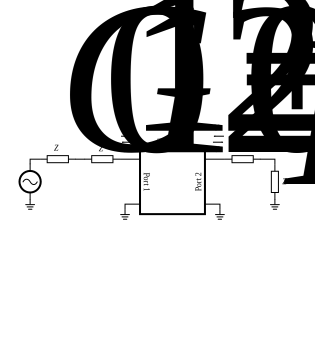
\includegraphics{img/analysis/s_parameter_twoport}
    \caption{S-parameters of a two-port system.}
    \label{fig:twoport}
\end{figure}

The reflection coefficient, $\Gamma$, can more generally be described as an \emph{S-parameter}. The S-parameters describe the ratio between the reflected and incident wave at a given port in a system. Consider a two-port as shown in Figure~\ref{fig:twoport}. Its four S-parameters are defined as follows:
\begin{align*}
    &S_{11} = \frac{V_1^-}{V_1^+} \Bigg|_{V_2^+=0} = \Gamma_1
    &&S_{12} = \frac{V_1^-}{V_2^+} \Bigg|_{V_1^+=0} \\
    &S_{21} = \frac{V_2^-}{V_1^+} \Bigg|_{V_2^+=0}
    &&S_{22} = \frac{V_2^-}{V_2^+} \Bigg|_{V_1^+=0} = \Gamma_2
\end{align*}
It is seen that $S_{11}$ and $S_{22}$ indicate the reflection due to the incident wave on the same port, when no contribution is made from the opposite port, i.e., these are the reflection coefficients of port 1 and 2, respectively. The parameter $S_{21}$ indicates how much of the incident wave on port 1 is coming out of port 2 when no wave is incident on port 2, i.e., this indicates the \emph{transmission coefficient} from port 1 to port 2. Likewise, $S_{12}$ is the transmission coefficient from port 2 to port 1.

The S parameters are easily measured using a Vector Network Analyzer (VNA). The advantage of measuring S-parameters over, e.g., Y-parameters is that all ports are matched during the measurement instead of some being shorted, making odd behavior (like oscillations) less likely \cite{Bowick2007}.

% Smith chart visualization
\begin{figure}[htbp]
    \centering
    \begin{tikzpicture}
        \begin{smithchart}
            \addplot coordinates {(3,0)};
            \path[draw=red] (0pt,0pt) circle (14.4mm);
        \end{smithchart}
    \end{tikzpicture}
    \caption{Smithchart. \fixme{SWR line not accurate\ldots}}
    \label{fig:smithchart}
\end{figure}
An important tool when doing matching, and designing antennas, to a certain $Z_0$ is the smith chart. The smith chart is used for plotting complex, normalized impedances and makes it easy to visually analyze the performance of a matched circuit. A smith chart is shown in Figure~\ref{fig:smithchart}.

The smith chart maps the entire right complex half-plane into a circle, having $0+j0$ all the way to the left and $\infty+j0$ all the way to the right. The y-axis (crossing $x=0$) makes up the circumference of the circle. An impedance is plotted by first finding the resistive (real) part of the impedance on the horizontal line and then following the circular grid-lines up or down for positive or negative reactances, respectively. 

The smith chart shown in Figure~\ref{fig:smithchart} is a normalized smith chart. When matching to $Z_0$, any impedance, $Z$, plotted in the smith chart, must be normalized by $Z_0$:
\begin{equation}
    Z_n = \frac{Z}{Z_0}
\end{equation}
This means that $Z_0$ will always appear at $1+j0$ -- in the center -- of the smith chart, and the goal of the matching is to get the impedance of the antenna (or other circuitry) as close to the center as possible for the desired frequency range.

The impedance bandwidth of an antenna is often given as the bandwidth for which the reflection coefficient, $\Gamma$, is below 0.5 (or \SI{-6}{dB}). It may therefore be advantageous to plot this requirement. In the smith chart, this is plotted as a circle around the center and any point within the circle, is within the bandwidth of the circuit. The \SI{-6}{dB} circle is also shown in Figure~\ref{fig:smithchart}.

% Matching circuitry, L-network, smith chart ``ups and downs'', analytical formulas.

% Tuners: Series capacitor, shunt capacitor, variable inductor?

% Insertion loss, S21 for networks, equivalent series resistance, component Q.

\section{LTE}
In this part an overview of the allocated LTE frequency bands will be provided together with a general description of the lte spectrum.
Furthermore in addition to the allocated LTE bands a more detailed description on the bands covered in this project will be provided.

LTE (Long Term Evolution) is an evolution of the UMTS (Universal Mobile Telecommunications System), HSPA (High Speed Packet Access) and HSPA+ (Evolved High Speed Packet Access) 3G communication standards. HSPA and HSPA+ are upgrades to UMTS for the primary goal to provide higher data rates. The LTE is advertised as a 4G network first commercial services was introduced in 2009 
 
\subsection{LTE Frequency Band Allocation}
\begin{table}[]
\centering
\caption{LTE frequency band allocation \cite{radio2015electronics}}
\label{table:ltefreqband}
\begin{tabular}{|c|c|c|c|c|c|}
\hline
\begin{tabular}[c]{@{}c@{}}LTE\\ band\\ number\end{tabular} & \begin{tabular}[c]{@{}c@{}}Uplink\\ (MHz)\end{tabular} & \begin{tabular}[c]{@{}c@{}}Downlink\\ (MHz)\end{tabular} & \begin{tabular}[c]{@{}c@{}}Width\\ of\\ band \\ spacing\end{tabular} & \begin{tabular}[c]{@{}c@{}}Duplex\\ spacing\\ (MHz)\end{tabular} & \begin{tabular}[c]{@{}c@{}}Band \\ Gap\\ (MHz)\end{tabular} \\ \hline
1                                                           & 1920 - 1980                                            & 2110 - 2170                                              & 60                                                                   & 190                                                              & 130                                                         \\ \hline
2                                                           & 1850 - 1910                                            & 1930 - 1990                                              & 60                                                                   & 80                                                               & 20                                                          \\ \hline
3                                                           & 1710 - 1785                                            & 1805,-1880                                               & 75                                                                   & 95                                                               & 20                                                          \\ \hline
4                                                           & 1710 - 1755                                            & 2110 - 2155                                              & 45                                                                   & 400                                                              & 355                                                         \\ \hline
5                                                           & 824 - 849                                              & 869 - 894                                                & 25                                                                   & 45                                                               & 20                                                          \\ \hline
6                                                           & 830 - 840                                              & 875 - 885                                                & 10                                                                   & 35                                                               & 25                                                          \\ \hline
7                                                           & 2500 - 2570                                            & 2620 - 2690                                              & 70                                                                   & 120                                                              & 50                                                          \\ \hline
8                                                           & 880 - 915                                              & 925 - 960                                                & 35                                                                   & 45                                                               & 10                                                          \\ \hline
9                                                           & 1749.9 - 1784.9                                        & 1844.9 - 1879.9                                          & 35                                                                   & 95                                                               & 60                                                          \\ \hline
10                                                          & 1710 - 1770                                            & 2110 - 2170                                              & 60                                                                   & 400                                                              & 340                                                         \\ \hline
11                                                          & 1427.9 - 1452.9                                        & 1475.9 - 1500.9                                          & 20                                                                   & 48                                                               & 28                                                          \\ \hline
12                                                          & 698 - 716                                              & 728 - 746                                                & 18                                                                   & 30                                                               & 12                                                          \\ \hline
13                                                          & 777 - 787                                              & 746 - 756                                                & 10                                                                   & -31                                                              & 41                                                          \\ \hline
14                                                          & 788 - 798                                              & 758 - 768                                                & 10                                                                   & -30                                                              & 40                                                          \\ \hline
15                                                          & 1900 - 1920                                            & 2600 - 2620                                              & 20                                                                   & 700                                                              & 680                                                         \\ \hline
16                                                          & 2010 - 2025                                            & 2585 - 2600                                              & 15                                                                   & 575                                                              & 560                                                         \\ \hline
17                                                          & 704 - 716                                              & 734 - 746                                                & 12                                                                   & 30                                                               & 18                                                          \\ \hline
18                                                          & 815 - 830                                              & 860 - 875                                                & 15                                                                   & 45                                                               & 30                                                          \\ \hline
19                                                          & 830 - 845                                              & 875 - 890                                                & 15                                                                   & 45                                                               & 30                                                          \\ \hline
20                                                          & 832 - 862                                              & 791 - 821                                                & 30                                                                   & -41                                                              & 71                                                          \\ \hline
21                                                          & 1447.9 - 1462.9                                        & 1495.5 - 1510.9                                          & 15                                                                   & 48                                                               & 33                                                          \\ \hline
22                                                          & 3410 - 3500                                            & 3510 - 3600                                              & 90                                                                   & 100                                                              & 10                                                          \\ \hline
23                                                          & 2000 - 2020                                            & 2180 - 2200                                              & 20                                                                   & 180                                                              & 160                                                         \\ \hline
24                                                          & 1625.5 - 1660.5                                        & 1525 - 1559                                              & 34                                                                   & -101.5                                                           & 135.5                                                       \\ \hline
25                                                          & 1850 - 1915                                            & 1930 - 1995                                              & 65                                                                   & 80                                                               & 15                                                          \\ \hline
26                                                          & 814 - 849                                              & 859 - 894                                                & 30/40                                                                &                                                                  & 10                                                          \\ \hline
27                                                          & 807 - 824                                              & 852 - 869                                                & 17                                                                   & 45                                                               & 28                                                          \\ \hline
28                                                          & 703 - 748                                              & 758 - 803                                                & 45                                                                   & 55                                                               & 10                                                          \\ \hline
29                                                          & n/a                                                    & 717 - 728                                                & 11                                                                   &                                                                  &                                                             \\ \hline
30                                                          & 2305 - 2315                                            & 2350 - 2360                                              & 10                                                                   & 45                                                               & 35                                                          \\ \hline
31                                                          & 452.5 - 457.5                                          & 462.5 - 467.5                                            & 5                                                                    & 10                                                               & 5                                                           \\ \hline
\end{tabular}
\end{table}

From the table it is seen that the allocated LTE bands reaches from \SIrange{452.5}{3600}{MHz}, although the whole spectrum is not covered by the lte, as other communication systems as GSM (2G) and UMTS (3G) etc. also uses band in this frequency range.  

FDD, TDD -- 

broadcast television spectrum around \SI{600}{MHz} has been freed
\cite{Samantha2015tunableAntennas}

 -- Europe band 20, 3, 7 


\subsection{Covered Bands}
In this project the frequencies of interest are \SIrange{700}{960}{MHz}, \SIrange{1710}{2170}{MHz}, \SIrange{2300}{2400}{MHz} and \SIrange{2550}{2650}{MHz}, also as specified in the requirement specification.


\section{User Effects}
\label{se:user_effects}
In this section the user impact on mobile antenna performance will be described, including both effects of the head, hand and the body in general.


Antenna parameters such as efficiency, radiation pattern, impedance etc. will be effected by the user, as the body of the user will look like a lossy and large dielectric body from the antennas point of view. 
The internal antennas that are implemented in every phone today, have a similar performance compared to external stubby antennas, which were used in a numerous of older designs. However this is only if the antennas are measured and compared in free space or next to a phantom head. In practical use a mobile phone with an internal antenna design, will be much more vulnerable to head and hand impacts from the user. The negative performance impact will be there, but will differ from user to user, as things like head and hand size, characteristics, hold position, left or right hand etc. varies from different users. This is of course a drawback in switching from external to internal antennas, but the development also comes with a lot of advantages. The internal antenna provides robust design and normally has higher performance in mechanical tests, such as drop tests, wearing tests etc. as the antenna is placed inside the phone, thus making physical interaction impossible. 
To counteract and minimize the user effect problem to the internal antennas, some basic design guidelines can be followed.

\subsection{Design Guidelines}
An antenna that is placed in the top of the phone, will be more effected by the user in talk mode, as the antenna will be closer to the head. To avoide this a ground plane can be placed between the user and the head in order to create more isolation. However placing the antenna on top of the ground plane decreases the bandwidth significantly, which leads to a, increase in the antenna size to keep the required bandwidth. This is not a reliable solution in mobile phones, as the size requirement of the antennas are very strict as a result of recent phone designs, with bigger screens and smaller cases. A way to solve this problem is to place the antenna in the bottom of the antenna, thus lowering the user effect and makes is possible to place the antenna without the ground plane as isolation. This solution provides a certain ground clearence, which makes it possible to decrease the volume and thickness of the antenna, thus saving place in the mobile phone. 
This design was proven to work by Motorola with there Motorola Razor V3 phone, which was the first phone to use the bottom placed antenna. There were some skeptics to this design, as the bottom of the phone would be placed in the middle of the hand in talk mode. However Motorola proved that theory wrong and therefore many phone manufactors are using there own bottom placed antennas. This solution of course only applies in talk mode, as the head effect is close to zero, when the phone is used in data mode. In data mode the phone is usually held either in horizontal mode with one hand or in vertical mode with two hands. In horizontal mode, given the size of today's smartphones, the hand will be placed around the middle of the phone (depending on the individual user), thus clearing the top and bottom. This indicates that it does not matter whether the antenna is placed in the top or bottom of the phone. In the case of horizontal mode with two hands, the hands covers both the top and the bottom of the phone, 
so in this case it still makes no difference if the antenna is placed in the bottom or in the top of the phone. 


In talk or data (horizontal or vertical) mode, there will still be some negative user effect on the performance. As long as the head or hand is within the near field of the phone, the impact of the user will be significant and needs some attention. Besides following the simple design guidelines, antenna tuning can be used to optimize the performance, when the antennas center frequency is detuned, as a result of the user impact.

\subsection{Recent Measurements}
A recent studie has been carried out in 2014 on user effects of MIMO LTE performance, which is also the antenna design goal of this project. The study is based on time-domain simulations of the user effects of head and hand phantoms in a free space scenario. The phantom hand used is modified, such that the finger can move across the phones backplane, to give more realistic results. The simulations is done in CST (Computer Simulation Technology) using the time-domain solver using FEM (Finite Element Method). Furthermore the antenna is placed in different positions, to evaluate on the user effect for different antenna positions. The different positions and the results of the simulation study, can be seen in Table \ref{tab:usereff_s11} and Table \ref{tab:usereff_radeff}. In Table \ref{tab:usereff_s11} the S-Parameter $S_{11}$ and $S_{22}$ are the reflection coefficient for the antenna at port 1 and 2 respectively and the $S_{21}$ results indicated the correlation between the two antennas. From the results it is clearly seen that the antennas is significally de-tuned in the presens of a user. In the worst case, the reflection coefficient drops from \SI{-8.2}{dB} to \SI{-0.6}{dB}, which is the case for the side mounted antenna. The bottom mounted antenna is the best case, where the reflection coefficient only drops approx. \SI{-2.5}{dB}, which is still a noticable drop. The correlation between the antennas

Finger position !    

\begin{table}[]
  \centering
  \begin{tabular}{|c|c|c|c|c|c|c|}
    \hline
    & \multicolumn{3}{c|}{\textbf{Antennas: Top/Side}} & \multicolumn{3}{c|}{\textbf{Antennas: Bottom/Side}} \\ \hline
                & $S_{11}$        & $S_{22}$        & $S_{21}$       & $S_{11}$         & $S_{22}$         & $S_{21}$             \\ \hline
    \textbf{FS} & -7.9           & -8.2           & -8.4           & -7.9            & -8.2            & -8.4            \\ \hline
    \textbf{P1} & -2.4           & -1.2           & -22.7          & -5.5            & -1.1            & -21.0           \\ \hline
    \textbf{P2} & -4.8           & -1.2           & -22.5          & -5.5            & -0.6            & -22.9           \\ \hline
    \textbf{P3} & -2.0           & -1.2           & -22.8          & -5.1            & -1.8            & -19.7           \\ \hline
    \textbf{P4} & -4.8           & -1.2           & -22.2          & -5.2            & -1.9            & -19.2           \\ \hline
    \textbf{P5} & -1.5           & -1.1           & -22.6          & -4.8            & -2.6            & -19.4           \\ \hline
    \textbf{P6} & -4.3           & -1.1           & -22.5          & -5.0            & -2.0            & -18.5           \\ \hline
  \end{tabular}
  \caption{S-parameter of the two MIMO antennas in free space compared to the user effect of the hand in six different finger positions \cite{Samantha2014UserEff}}
  \label{tab:usereff_s11}
\end{table}

\begin{table}[]
\centering
\begin{tabular}{|c|c|c|c|c|c|c|c|c|}
\hline
            & \multicolumn{4}{c|}{\textbf{Antennas: Top/Side}} & \multicolumn{4}{c|}{\textbf{Antennas: Bottom/Side}} \\ \hline
            & R1         & R2        & T1         & T2         & R1         & R2          & T1         & T2          \\ \hline
\textbf{FS} & -0.2       & -1.1      & -1,0       & -1,9       & -0.2       & -1.1        & -1.0       & -1.9        \\ \hline
\textbf{P1} & -13.4      & -9.2      & -15.8      & -14.8      & -8.9       & -10.9       & -9.6       & -17.0       \\ \hline
\textbf{P2} & -14.1      & -8.6      & -14.7      & -14.6      & -8.6       & -9.7        & -9.0       & -18.5       \\ \hline
\textbf{P3} & -13.3      & -9.3      & -16.2      & -14.9      & -8.7       & -14.4       & -9.7       & -18.5       \\ \hline
\textbf{P4} & -14.3      & -8.9      & -14.9      & -14.9      & -8.6       & -14.4       & -9.6       & -18.2       \\ \hline
\textbf{P5} & -14.0      & -9.6      & -17.6      & -15.5      & -8.9       & -15.2       & -9.9       & -18.8       \\ \hline
\textbf{P6} & -14.0      & -8.8      & -14.6      & -15.0      & -8.7       & -15.4       & -9.7       & -18.1       \\ \hline
\end{tabular}
\caption{Radiation and total efficiency of the two MIMO antennas in free space compared the user effect of the hand in six different finger positions \cite{Samantha2014UserEff}}
\label{tab:usereff_radeff}
\end{table}


User effects of MIMO LTE performance 2014 measurements. \cite{Samantha2014UserEff}
\section{Finite Difference Time Domain}
\label{sec:fdtd}
This section will describe the finite difference time domain method. This is a method for solving Maxwell equations in time domain. A brief introduction to Marxwell's Equations is given, in order to understand the methodology of FDTD. Then the teqniques and ideas behind FDTD are presenten and used on the 1D scalar wave-equation. Then an introduction to the Yee Algorithm, Yee cell and Yee notation is presenten and applied on the 3D Maxwell curl equation. Lastly the key parameters of FDTD are discussed and related to CST Microwavestudio.

\subsection{Introduction to Maxwell's Equations}
Maxwell's equations are a set of equations that describe how electric and magnetic fields propagate. The set of equations consists of Gauss' law, Gauss' Magnetism law, Faraday's law and finally Ampere's law. 

\subsubsection{Gauss' Law}
Gauss' law describes how the electric field behaves around electric charges. Below is Gauss' Law written in point differential-form, the equation states that the divergence of the electric flux density $\bold{D}$ is equal to the volume electric charge density $\rho_V$ \cite{taflove2000computional}. This is that the field around a point $\bold{D}$ is equal to electric charge density $\rho_V$. From this it is found that if there exists an electric charge, the divergence of $\bold{D}$ is nonzero, and only zero when there is no charge present. 

\begin{align}
\nabla \cdot \bold{D} &= \rho_V
\end{align}

\subsubsection{Gauss' Magnetism Law}
Gauss' magnetism law, is much like the previous formula, but for magnetic fields. Basically Gauss' law for magnetism states that a magnetic charge does not exist. This is given in the Equation below \cite{taflove2000computional}. 
\begin{align}
\nabla \cdot \bold{B} &=0
\end{align}
From this it is clear, that there are no magnetic monopoles, the divergence of $\bold{B}$ or $\bold{H}$ fields is always zero and that magnetic fields always flows in closed loops. 

\subsubsection{Faraday's Law}
Faraday's law states that the curl of the $\bold{E}$, is equal to the rate of change of a magnetic field. This is very important in the way that electric ways propagate. This is given in the Equation below \cite{taflove2000computional}. 
\begin{align}
\nabla \times \bold{E} &= - \frac{\partial \bold{B}}{\partial t}
\end{align}

From this equation, it can be seen that a time changing magnetic field gives rise to an E-field circulating around it. Likewise, a circulating E-field causes a time changing magnetic field.   

\subsubsection{Ampere's Law}
Ampere's law, is much like Faraday's law, but for curling magnetic fields. In simple words the Equation below stats that the curl of a magnetic field $\bold{H}$ is given by the rate of change of a electric field $\bold{D}$ termed displacement current density and the electric current density\cite{taflove2000computional}.

\begin{align}
\nabla \times \bold{H} &= \frac{\partial \bold{D}}{\partial t} + \bold{J} 
\end{align}
This is very much symmetric to Faraday's law, with an additional term. However the outcome is the same. That is that a time changing electric field gives rise to an H-field circulating around it and likewise a circulating H-field causes a time changing electric field. From Faraday and Ampere's law it is seen how waves can actually propagate, since a change in an electric field causes a curling magnetic field and so on.    

\subsubsection{Constitutive relations}
Before doing any mathematical manipulations or calculations, it is necessary to have an idea on how the different terms and variables are connected through physical constants. E.g. how the electric flux density is connected to the electric field, which can lead to simplification of calculations later on.

\paragraph{Electric Flux Density:} The electric flux density $\bold{D}$ is related to the electric field $\bold{E}$ by the permittivity measured in Farads per meter. Permittivity is a fundamental parameter of a given material, which affects the propagation of an electric field. Typically it is denoted by $\epsilon$. The relation is given by\cite{taflove2000computional}: 

\begin{align}
  \bold{D} = \epsilon \bold{E}
\end{align}

\paragraph{Magnetic Flux Density:} The magnetic flux density $\bold{B}$ is related to the magnetic field $\bold{H}$ by the permeability measured in Henries per meter. Permeability is a fundamental parameter of a given material, which affects the propagation of a magnetic field. Typically it is denoted by $\mu$. The relation is given by\cite{taflove2000computional}: 

\begin{align}
  \bold{B} = \mu \bold{H}
\end{align}
\paragraph{Electric Current Density:}  The electric current density $\bold{J}$ is related to the electric field $\bold{E}$ by the conductivity measured in Siemens per meter. Permeability is a fundamental parameter of a given material, which affects the current flow in a conductor. Typically it is denoted by $\sigma$. The relation is given by\cite{taflove2000computional}: 

\begin{align}
  \bold{J} = \sigma \bold{E}
\end{align}

\subsection{The 1D Wave Equation}
The wave equation is one of the most basic partial differential equation, which describes how waves propagate. This section will use the 1-dimension wave to describe the method of FDTD. Furthermore it is assumed that

\begin{itemize}
\item The region is free of charge and current: $\bold{J} = \bold{M} = 0$
\item The medium is linear (field-independent)
\item The medium is isotropic (direction-independent)
\item The medium is non-dispersive (frequency-independent)
\end{itemize}
Given these assumptions, Ampere's and Faraday's law can be rewritten as

\begin{align}
  \frac{\partial \epsilon \bold{E}}{\partial t} = \nabla \times \bold{H} - 0 & \implies \frac{\partial \bold{E}}{\partial t} = \frac{1}{\epsilon} \nabla \times \bold{H} \\
\frac{\partial \mu \bold{H}}{\partial t} =  - \nabla \times \bold{E} - 0 & \implies \frac{\partial \bold{H}}{\partial t} = - \frac{1}{\mu} \nabla \times \bold{E}
\end{align}
Expanding E- and H-field into the Cartesian components 

\begin{align}
  \frac{\partial E_x}{\partial t} = \frac{1}{\epsilon} \big(\frac{\partial H_z}{\partial y} - \frac{\partial H_y}{\partial t} \big) \qquad  
  \frac{\partial H_x}{\partial t} = \frac{1}{\mu} \big(\frac{\partial E_z}{\partial y} - \frac{\partial E_y}{\partial t} \big)\\
  \frac{\partial E_y}{\partial t} = \frac{1}{\epsilon} \big(\frac{\partial H_x}{\partial y} - \frac{\partial H_z}{\partial t} \big) \qquad 
  \frac{\partial H_y}{\partial t} = \frac{1}{\mu} \big(\frac{\partial E_x}{\partial y} - \frac{\partial E_z}{\partial t} \big) \\
  \frac{\partial E_z}{\partial t} = \frac{1}{\epsilon} \big(\frac{\partial H_y}{\partial y} - \frac{\partial H_x}{\partial t} \big) \qquad 
  \frac{\partial H_z}{\partial t} = \frac{1}{\mu} \big(\frac{\partial E_y}{\partial y} - \frac{\partial E_x}{\partial t} \big)
\end{align}
which for the 1D case $\frac{\partial}{\partial z} = \frac{\partial}{\partial y} = 0$ simplifies to 

\begin{align}
  \frac{\partial E_x}{\partial t} &= 0 \\
  \frac{\partial E_y}{\partial t} &= - \frac{1}{\epsilon} \frac{\partial H_z}{\partial x}\\
  \frac{\partial E_z}{\partial t} &= \frac{1}{\epsilon} \frac{\partial H_y}{\partial x}
\end{align}
The same steps can be used to get an expression for the H-field. For each direction we can combine the E and H expressions to get the 1D scalar wave equation, e.g. the z-direction\cite{taflove2000computional}: 

\begin{align}
  \frac{\partial^2 E_z}{\partial t^2} = c^2 \frac{\partial^2 E_z}{\partial x^2}
\end{align}
Where $c$ is the speed of light. This equation tells us that an electric field moving in the z-direction, will propagate along the x-axis in time, with a speed of $c$. Going back to the general wave-equation\cite{taflove2000computional}

\begin{align}
  \frac{\partial^2 u}{\partial t^2} = c^2 \frac{\partial^2 u}{\partial x^2}
\end{align}
Since the wave-equation is a second order partial differential equation, it is known to have two linearly independent solutions\cite{taflove2000computional}: 

\begin{align}
  u(x,t) = F(x+ct) + G(x-ct)
\end{align}
Both $F$ and $G$ are known as propagating-wave solutions, where an argument of the form $x+ct$ is a wave moving towards decreasing $x$ and an argument of the form $x-ct$ is a wave moving towards increasing $x$\cite{taflove2000computional}. In order to compute this numerically finite differences are used. Thus the following needs to be approximated using finite-differences 

\begin{align}
  \frac{\partial^2 u(x,t)}{\partial t^2},\frac{\partial^2 u(x,t)}{\partial x^2}
\end{align}

Taylor series expansion is used to approximate the expression at a point $x_i$ using finite differences: $u(x_i) = u(x_i+\Delta x) + u(x_i - \Delta x)$ which then is used to solve the wave-equation by substituting the two central differences into the 1D wave equation. This gives the solution for the latest time step as\cite{taflove2000computional}

\begin{align*}
  u_i^{n+1} =& \left( \frac{c\Delta t}{\Delta x} \right) \left[ u_{i+1}^n - 2u_i^n + u_{i-1}^n \right] + 2u_i^n -u_i^{n-1} \\
             &+ O[(\Delta t)^2] + O[(\Delta x)^2]
\end{align*}

\subsection{Dispersion}
When ever discrete numerical methods are used dispersion must be taken into account. Dispersion in this case can be seen as a variation in wavelength. For the wave equation this depends on the chosen time and space steps\cite{taflove2000computional}. 

\begin{itemize}
\item \textbf{Magic time-step:} $c\Delta t = \Delta x$. No dispersion.
\item \textbf{Very fine mesh:} $\Delta t \rightarrow 0$, $\Delta x \rightarrow 0$. No dispersion.
\item \textbf{Difference 1:} $c\Delta t < \Delta x$. Wavelength smaller in sampled space than in reality.
\item \textbf{Difference 2:} $c\Delta t > \Delta x$. Unstable as $\omega$ is complex. Exponential growth.
\end{itemize}

Generally the magic time-step is only an exact solution in 1D, but it exists for all dimensions but only for one incident angle\cite{taflove2000computional}. It is also seen that finer mesh cells reduces the error term.  

\subsection{The Yee Algorithm}
The Yee algorithm is a set of finite difference equations for Maxwell's curl equation system derived by Kane Yee. This algorithm solves both E- and H-fields in space and time using coupled curl equations instead of solving for one field at a time using the wave equation. Some of the key features of the Yee Algorithm is\cite{taflove2000computional}

\begin{itemize}
\item Both E- and H-field boundaries can be used
\item Solving both E- and H-fields is more robust 
\item Electric and magnetic material properties can be modeled easily
\item Unique field features, e.g. singularities. 
\end{itemize}
The Yee algorithm centers the E- and H-fields in 3D, such that every E-field is surrounded by four curling H-fields and every H-field is surrounded by four curling E-fields. This is illustrated on Figure~\ref{fig:fdtd-grid}, each cell referred to as the Yee-cell, a single Yee cell is shown in Figure~\ref{fig:yee-cell}. The arrangement of the electric and magnetic fields implicitly enforce Gauss' Law and Gauss' Magnetic Law, which makes the Yee mesh divergence free with respect to the E- and H-fields\cite{taflove2000computional}.  

\begin{figure}
    \centering
    \begin{subfigure}[b]{0.49\textwidth}
      \centering
        \includegraphics[scale=0.3]{img/analysis/fdtd_mesh}
        \caption{A Yee FDTD grid}
        \label{fig:fdtd-grid}
    \end{subfigure}
    ~
    \begin{subfigure}[b]{0.49\textwidth}
      \centering
        \includegraphics[scale=0.7]{img/analysis/yee_3d}
        \caption{A single Yee cell}
        \label{fig:yee-cell}
    \end{subfigure}
    \caption{Spatial interpetation of the Yee Algorithm}
    \label{fig:space-yee-algorithm}
\end{figure}

The centering of the E- and H-fields in time, is often termed the leapfrog method. This time stepping is fully explicit, and thus avoiding problems with simultaneous equations and matrix inversion. This leapfrog method is shown on Figure~\ref{fig:leap_frog} 

\begin{figure}[htbp]
    \centering
    \includegraphics[scale=0.7]{img/analysis/leap_frog}
    \caption{Leap-frog method illustrated on the time line}
    \label{fig:leap_frog}
\end{figure}

To keep an overview Yee, created the following notation which is useful when considering 3D FDTD equations

\begin{align}
  u_X (i \Delta x , j \Delta y, k \Delta z, n \Delta t) = u^n_{X_{i,j,k}}
\end{align}

%http://www.ualr.edu/wirelesslab/fdtd/fdtd3.pdf
\subsubsection{Finite Difference of Maxwell's Equations in 3D}
For completeness the previous ideas and notation can now be used to derive a numerical approximation of Maxwell's Curl Equations in 3D. The derivations will not be shown here, and only the solution for a single Cartesian component will be given here, due to its complexity. As an example the approximation for $E_x$ is shown below\cite{taflove2000computional}: 

\begin{align}
  &E_x |^{n+1/2}_{i,j+1/2,k+1/2} = \big( \frac{1-\frac{\sigma_{i,j+1/2,k+1/2} \Delta t}{2\epsilon_{i,j+1/2,k+1/2}}}{1+\frac{\sigma_{i,j+1/2,k+1/2} \Delta t}{2\epsilon_{i,j+1/2,k+1/2}}} \big) E_x |^{n-1/2}_{i,j+1/2,k+1/2}  + \\ &\big(  \frac{\frac{\Delta t}{\epsilon_{i,j+1/2,k+1/2}}}{1+\frac{\sigma_{i,j+1/2,k+1/2} \Delta t}{2\epsilon_{i,j+1/2,k+1/2}} }    \big) \big( \frac{H_z |^n_{i,j+1,k+1/2} - H_z |^n_{i,j,k+1/2} }{\Delta y} - \frac{H_y |^n_{i,j+1/2,k+1} - H_y |^n_{i,j+1/2,k} }{\Delta z} -J_{source}|^n_{i,j+1/2,k+1/2}  \big)
\end{align}

As seen the equations quickly become large and hard to handle, however to fully extend this to 3D this would have to be done for all the the Cartesian coordinates for both E- and H-fields. 

\subsection{Absorbing Boundary Conditions}
Since many geometries of interest are defined in open regions, e.g. antennas, where the spatial domain is unbounded. Since computers have limited storage, it is needed to find a suitable boundary condition on the outer perimeter of the domain $\Omega$ in order to simulate to infinity. Thus it is needed to find a boundary condition that allows outward propagating numerical wave to exit the outer perimeter of $\Omega$, without spurious reflections from the outgoing waves. 

One way of achieving the absorbing boundary condition is by terminating the outer boundary with an absorbing material, which is analogous to the method used in anechoic chambers. For this perfectly matched layer (PML) is used, which is derived by Berenger. This allows plane waves of arbitrary incidence, polarization and frequency to be matched at the boundary. PML usually gives a back-reflection in the order of $\approx 10^{-6}$--$10^{-8}$.\cite{taflove2000computional}

\subsection{FDTD Parameters and Relation to CST}
For all simulations in this report CST microwave studio is being used. The following will try to connect the FDTD theory to the parameters in CST. Even though CST uses Finite Integration Technique (FIT) instead of finite differences. FIT share the structure of FDTD, but using the Maxwell's Equations on integral form. The advantage of FIT is that is uses less memory and it is allows for easier code implementation of some features. Besides this most of the basic parameters are the same. 

\subsubsection{Cell Size and Meshing}
The coice of cell size is very important when doing FDTD simulations. A general rule of thumb is that a cell should be much less than the smallest wavelength, it is often said that 10 cells per wavelength is sufficient, that is the cell size should be $\lambda/10$. In advanced FDTD simulations an adaptive meshing is often used, where even smaller cells are used in dense materials with high field locations, and then large cells outside these areas. When doing this it is also very important not to change the cell size too much compared to the neighbor cells. It is also important
that the cell size are small enough to approximate the geometry which is to be modeled accurately. Geometries such as circles are being approximated with rectangular cells, this causes a ``staircase effect'' on the object, and the representation can be inaccurate if the cell sizes used are too large. 

Another rule of thumb, which can help assessing the right cell size is that the smallest mechanical item of the structure is to be approximated by at least two cells. The rule of thumb says that\cite{kunz1993fdtd}:
\begin{align}
    \Delta = \frac{d_{\text{min}}}{N_d} 
\end{align}
where 
\begin{where}
\item[$\Delta$] Is the length/width/height of the cell.
\item[$d_{\text{min}}$] Smallest physical dimension.
\item[$N_d$] Oversampling factor -- should be $\geq 1$.
\end{where}


\subsubsection{Time Step Size}
The time step size is another parameter that has to be chosen with care, when doing FDTD simulations. The time step should be small enough, such that at any point a wave should not pass through more than one cell.  Calculating the time step is dependent on the cell size and dimensions and the propagation speed.  The time step for the 3D rectangular grid can be calculated as:
\begin{align}
   \Delta t &= \frac{1}{c \sqrt{\frac{1}{(\Delta x)^2}+\frac{1}{(\Delta y)^2}+\frac{1}{(\Delta z)^2}}} \\
            &= \frac{1}{c \sqrt{\frac{3}{\Delta^2}}} \\
            &= \frac{\Delta}{c \sqrt{3}} \label{eq:deltat}           
\end{align}
where:
\begin{where}
\item [$c$] Speed of light.
\item [$\Delta = \Delta x = \Delta y = \Delta z$] Size of the cell side for rectangular cell.
\end{where}
The step size should also be reduced for the materials with conductivity higher then zero. If the time step is chosen to be larger than given in Equation~\ref{eq:deltat} instabilities can occur \cite{kunz1993fdtd}.   

\subsubsection{Accuracy and time limit}
These terms are taking from CST microwave studio, and are figures that limit the simulation either when a certain accuracy criteria has been met or when it has been simulation for a certain amount of time. In practice it is not wanted that a simulation is to be stopped due to a given time limit, therefor this limit is often set to a very large number. In CST accuracy is a figure that describes how much energy is left in the system. The accuracy setting stops the simulation when a certain energy level within the structure has decreased to a chosen level. 

\section{Problem Statement}
\label{sec:problem_statement}
The problem statement, which will be investigated in this report, is formulated as the following:
\begin{quote}
    \itshape
    How can a pair of MIMO antennas for LTE handsets be designed so that all bands from \SI{700}{MHz} to \SI{960}{MHz} and from \SI{1710}{MHz} to \SI{2650}{MHz} are covered with a total efficiency above \SI{50}{\%} using a tunable MEMS capacitor, and how does a small ground clearance -- the distance between the antenna element and the ground plane -- affect the performance?
\end{quote}
The further specifications for the design will be described next in the requirement specification.


% Requirements
\chapter{Requirements Specification}
\label{cha:reqspec}

\section{Functional Requirements}
\noindent
\begin{tabularx}{\linewidth}{|l|X|}
    \hline
    ID & Requirement \\
    \hline
    \freq{dualband} & The antenna system must consist of two single-feed dual-band antennas covering the bands described in Requirement~\sreqref{fbands}. \\
    \freq{updownlink} & Each antenna must cover both uplink and downlink at the same time for each required LTE band.\\
    \freq{usereffect} & Must be able to re-tune any detuning due to user effects. \\
    \freq{matching} & Must have a simple matching network, containing a variable capacitor for tuning inside the specified bands.\\
    \freq{wispry} & Must use a wiSpry WS1040 MEMS variable capacitor chip in the matching network.\\
    \hline
\end{tabularx}

\section{Specific Requirements}
\noindent 
\begin{tabularx}{\linewidth}{|l|l|X|}
    \hline
    ID & Specification & Requirement \\
    \hline
    \sreq{fbands} & Frequency bands\slash tunable range & \num{700}--\SI{960}{MHz}, \num{1710}--\SI{2170}{MHz}, \num{2300}--\SI{2400}{MHz}, \num{2550}--\SI{2650}{MHz} \\
    \sreq{bandwidthlow} & Minimum tunable bandwidth (\num{700}--\SI{960}{MHz}) & \SI{80}{MHz} (band 8) \\
    \sreq{bandwidthhigh} & Minimum tunable bandwidth (\num{1710}--\SI{2650}{MHz}) & \SI{720}{MHz} (band 15) \\
    \sreq{physdim} & Physical dimensions & External: $70\times140\times7$\,\si{mm\cubed}, PCB: $55\times120\times1.6$\,\si{mm\cubed} (FR-4)\\
    \sreq{copper} & Ground plane copper thickness & \SI{0.035}{mm} \\
    \sreq{retloss} & In-band return loss (impedance bandwidth) & $\text{RL} > \SI{6}{dB}$\\
    \sreq{correlation} & In-band correlation between antenna elements (correlation bandwidth) & $\rho_e < 0.5$\\
    \sreq{efficiency} & In-band total efficiency in free-space (efficiency bandwidth)  & $>\SI{50}{\%}$ \\
    \sreq{sar} & Maximum SAR & \SI{2}{W\per kg} averaged over \SI{10}{g} of tissue\\
    \sreq{tunable} & Tunable capacitor range (WS1040)& \SI{0.3}{pF} to \SI{2.9}{pF} in steps of \SI{0.2}{pF} (\SI{0.1}{pF} minimum)  \\
    \sreq{ltepower} & Reference power level  & \SI{23}{dBm} (\SI{0.2}{W})\\
    \hline
\end{tabularx}



% Technical solution

% Back matter %%%%%%%%%%%%%%%%%%%%%%%%%%%%%%%%%%%%%%%%%%%%%%%%%%%%%%%%%%%%%%%%%%
\listoffixmes
\bibliographystyle{ieeetr}
\bibliography{bib/sources}
\addcontentsline{toc}{chapter}{Bibliography}

\end{document}
